\documentclass[titlepage]{article}
\usepackage{amsmath}
\usepackage{algorithm}
\usepackage{algpseudocode}
\usepackage{listings}
\usepackage{enumerate}
\usepackage{graphicx}
\usepackage{xcolor}
\usepackage{fancyhdr}

\lstset{
    language=C++,
    basicstyle=\ttfamily\small,
    numbers=left,
    numberstyle=\tiny,
    frame=single,
    breaklines=true,
    keywordstyle=\color{blue},
    commentstyle=\color{green!60!black},
    stringstyle=\color{red},
    showstringspaces=false
}

\graphicspath{{./images/}}

\title{BCSE309P - Cryptography \& Network Security Lab \\ 
\textbf{Lab Assignment 1}}
\author{Kedar Shinde 22BCE1765}
\date{}

\begin{document}
\pagestyle{fancy}
\fancyhead{} % clear all header fields
\fancyhead[RO,LE]{\textbf{Lab Assignment 1}}
\fancyhead[RE,LO]{\textbf{BCSE309P}}
\fancyfoot{} % clear all footer fields
\fancyfoot[LE,RO]{\thepage}
\fancyfoot[LO,RE]{\textbf{Kedar Shinde 22BCE1765}}
\maketitle

\section{Aim}
To implement the Caesar cipher, Vigenère cipher, Vernam cipher, Playfair cipher, Hill cipher, and Columnar transposition cipher.

\section{Steps for Encryption and Decryption}
\subsection{Caesar Cipher}
The Caesar cipher, named after Julius Caesar, is a substitution cipher that shifts each letter in the plaintext by a fixed number of positions in the alphabet.

\subsubsection{ Steps for Encryption}
\begin{enumerate}[1.]
\item For each character in the plaintext message:
   \begin{enumerate}[a)]
   \item Check if the character is alphabetic using \texttt{isalpha()}
   \item Determine the base value:
      \begin{itemize}
      \item If lowercase: base = 'a' (97 in ASCII)
      \item If uppercase: base = 'A' (65 in ASCII)
      \end{itemize}
   \item Apply the shift transformation:
      \begin{equation}
      E(c) = (c - \text{base} + \text{shift}) \bmod 26 + \text{base}
      \end{equation}
   \item Non-alphabetic characters remain unchanged
   \end{enumerate}
\end{enumerate}

\subsubsection{ Steps for Decryption}
\begin{enumerate}[1.]
\item For each character in the ciphertext:
   \begin{enumerate}[a)]
   \item Check if the character is alphabetic
   \item Determine the base value (same as encryption)
   \item Apply the reverse shift:
      \begin{equation}
      D(c) = (c - \text{base} - \text{shift} + 26) \bmod 26 + \text{base}
      \end{equation}
   \item The +26 ensures positive modulus result
   \end{enumerate}
\end{enumerate}

\subsection{Vigenère Cipher}
The Vigenère cipher enhances the Caesar cipher by using a keyword to create multiple shift values, making it more resistant to frequency analysis.

\subsubsection{Key Generation Process}
\begin{enumerate}[1.]
\item Calculate required key length:
   \begin{equation}
   \text{required\_length} = \text{message\_length}
   \end{equation}
\item Generate repeating key:
   \begin{enumerate}[a)]
   \item Calculate complete repetitions: $\text{reps} = \lfloor\frac{\text{message\_length}}{\text{key\_length}}\rfloor$
   \item Calculate remaining characters: $\text{remainder} = \text{message\_length} \bmod \text{key\_length}$
   \item Repeat key \texttt{reps} times
   \item Append first \texttt{remainder} characters of key
   \end{enumerate}
\end{enumerate}

\subsubsection{ Encryption Steps}
\begin{enumerate}[1.]
\item Generate the extended key to match message length
\item For each character position $i$:
   \begin{enumerate}[a)]
   \item Get plaintext character $p_i$ and key character $k_i$
   \item If $p_i$ is alphabetic:
      \begin{itemize}
      \item Determine character case and base
      \item Apply Vigenère transformation:
         \begin{equation}
         E(p_i) = ((p_i - \text{base} + (k_i - \text{base})) \bmod 26) + \text{base}
         \end{equation}
      \end{itemize}
   \item Preserve non-alphabetic characters
   \end{enumerate}
\end{enumerate}

\subsubsection{ Decryption Steps}
\begin{enumerate}[1.]
\item Generate the same extended key
\item For each character position $i$:
   \begin{enumerate}[a)]
   \item Get ciphertext character $c_i$ and key character $k_i$
   \item If $c_i$ is alphabetic:
      \begin{itemize}
      \item Determine character case and base
      \item Apply reverse transformation:
         \begin{equation}
         D(c_i) = ((c_i - \text{base} - (k_i - \text{base}) + 26) \bmod 26) + \text{base}
         \end{equation}
      \end{itemize}
   \end{enumerate}
\end{enumerate}

\subsection{Vernam Cipher}
The Vernam cipher, also known as the one-time pad when used with a truly random key, provides perfect secrecy when implemented correctly.

\subsubsection{Key Requirements}
\begin{enumerate}[1.]
\item Key length must equal or exceed message length
\item Key should ideally be truly random
\item Key must never be reused
\end{enumerate}

\subsubsection{ Encryption Steps}
\begin{enumerate}[1.]
\item Validate key length against message length
\item For each character position $i$:
   \begin{enumerate}[a)]
   \item Perform bitwise XOR operation:
      \begin{equation}
      \text{temp} = p_i \oplus k_i
      \end{equation}
   \item Ensure printable ASCII result:
      \begin{equation}
      E(p_i) = \text{temp} \& 0x7F
      \end{equation}
   \end{enumerate}
\end{enumerate}

\subsubsection{ Decryption Steps}
\begin{enumerate}[1.]
\item For each character position $i$:
   \begin{enumerate}[a)]
   \item Perform bitwise XOR with same key:
      \begin{equation}
      \text{temp} = c_i \oplus k_i
      \end{equation}
   \item Ensure printable ASCII:
      \begin{equation}
      D(c_i) = \text{temp} \& 0x7F
      \end{equation}
   \end{enumerate}
\end{enumerate}

\subsection{Playfair Cipher}
The Playfair cipher encrypts pairs of letters using a 5×5 matrix constructed from a keyword.

\subsubsection{ Key Matrix Generation}
\begin{enumerate}[1.]
\item Process the keyword:
   \begin{enumerate}[a)]
   \item Remove duplicate characters
   \item Convert to lowercase
   \item Replace 'j' with 'i'
   \end{enumerate}
\item Create the alphabet string:
   \begin{enumerate}[a)]
   \item Use "abcdefghiklmnopqrstuvwxyz" (no 'j')
   \item Remove letters already in processed key
   \end{enumerate}
\item Construct 5×5 matrix:
   \begin{enumerate}[a)]
   \item Fill with processed key first
   \item Fill remaining positions with remaining alphabet
   \end{enumerate}
\end{enumerate}

\subsubsection{Plaintext Preprocessing}
\begin{enumerate}[1.]
\item Remove non-alphabetic characters
\item Convert to lowercase
\item Replace 'j' with 'i'
\item Split into digraphs (pairs):
   \begin{enumerate}[a)]
   \item If pair has same letters, insert 'x' between them
   \item If text length is odd, append 'x'
   \end{enumerate}
\end{enumerate}

\subsubsection{ Encryption Rules}
\begin{enumerate}[1.]
\item For each letter pair $(a,b)$:
   \begin{enumerate}[a)]
   \item Find positions $(row_1,col_1)$ and $(row_2,col_2)$ in matrix
   \item Apply transformation rules:
      \begin{itemize}
      \item Same row: $E(a) = M[row_1][(col_1+1)\bmod 5]$, $E(b) = M[row_2][(col_2+1)\bmod 5]$
      \item Same column: $E(a) = M[(row_1+1)\bmod 5][col_1]$, $E(b) = M[(row_2+1)\bmod 5][col_2]$
      \item Rectangle: $E(a) = M[row_1][col_2]$, $E(b) = M[row_2][col_1]$
      \end{itemize}
   \end{enumerate}
\end{enumerate}

\subsubsection{ Decryption Rules}
\begin{enumerate}[1.]
\item For each letter pair $(a,b)$:
   \begin{enumerate}[a)]
   \item Find positions in matrix
   \item Apply reverse transformations:
      \begin{itemize}
      \item Same row: $D(a) = M[row_1][(col_1-1)\bmod 5]$, $D(b) = M[row_2][(col_2-1)\bmod 5]$
      \item Same column: $D(a) = M[(row_1-1)\bmod 5][col_1]$, $D(b) = M[(row_2-1)\bmod 5][col_2]$
      \item Rectangle: $D(a) = M[row_1][col_2]$, $D(b) = M[row_2][col_1]$
      \end{itemize}
   \end{enumerate}
\end{enumerate}

\subsection{Hill Cipher}
The Hill cipher uses linear algebra for encryption, representing text using matrices and performing matrix multiplication.

\subsubsection{Matrix Operations}
\begin{enumerate}[1.]
\item Calculate matrix determinant:
   \begin{equation}
   \det(K) = k_{11}k_{22} - k_{12}k_{21}
   \end{equation}
\item Find modular multiplicative inverse:
   \begin{equation}
   \det(K)^{-1} \bmod 26 \text{ where } \det(K) \times \det(K)^{-1} \equiv 1 \pmod{26}
   \end{equation}
\item Calculate adjugate matrix:
   \begin{equation}
   adj(K) = \begin{bmatrix} 
   k_{22} & -k_{12} \\
   -k_{21} & k_{11}
   \end{bmatrix}
   \end{equation}
\end{enumerate}

\subsubsection{ Encryption Steps}
\begin{enumerate}[1.]
\item Preprocess plaintext:
   \begin{enumerate}[a)]
   \item Remove non-alphabetic characters
   \item Convert to lowercase
   \item Pad with 'x' if needed
   \end{enumerate}
\item Convert text to numbers (a=0, b=1, etc.)
\item For each block of n letters (n = matrix size):
   \begin{enumerate}[a)]
   \item Create column vector $P$
   \item Compute $C = KP \bmod 26$
   \item Convert result back to letters
   \end{enumerate}
\end{enumerate}

\subsubsection{ Decryption Steps}
\begin{enumerate}[1.]
\item Calculate inverse key matrix $K^{-1}$:
   \begin{equation}
   K^{-1} = \det(K)^{-1} \times adj(K) \bmod 26
   \end{equation}
\item For each block of n letters:
   \begin{enumerate}[a)]
   \item Create column vector $C$
   \item Compute $P = K^{-1}C \bmod 26$
   \item Convert result back to letters
   \end{enumerate}
\end{enumerate}

\subsection{Rail Fence Cipher (Columnar Transposition)}
The columnar transposition cipher rearranges characters based on the alphabetical ordering of a keyword.

\subsubsection{ Encryption Steps}
\begin{enumerate}[1.]
\item Calculate dimensions:
   \begin{enumerate}[a)]
   \item Number of columns = key length
   \item Number of rows = $\lceil\frac{\text{message\_length}}{\text{key\_length}}\rceil$
   \end{enumerate}
\item Create grid:
   \begin{enumerate}[a)]
   \item Fill grid row by row with plaintext
   \item Pad incomplete final row with spaces
   \end{enumerate}
\item Determine column order:
   \begin{enumerate}[a)]
   \item Number columns based on keyword letter positions
   \item Create mapping of column numbers to positions
   \end{enumerate}
\item Read off columns:
   \begin{enumerate}[a)]
   \item Read columns in order determined by key
   \item Ignore padding characters
   \end{enumerate}
\end{enumerate}

\subsubsection{ Decryption Steps}
\begin{enumerate}[1.]
\item Calculate dimensions (same as encryption)
\item Calculate column lengths:
   \begin{enumerate}[a)]
   \item Full columns: $\lfloor\frac{\text{message\_length}}{\text{key\_length}}\rfloor$
   \item Extra characters: $\text{message\_length} \bmod \text{key\_length}$
   \end{enumerate}
\item Reconstruct columns:
   \begin{enumerate}[a)]
   \item Determine original column order from key
   \item Place appropriate number of characters in each column
   \end{enumerate}
\item Read plaintext:
   \begin{enumerate}[a)]
   \item Read grid row by row
   \item Combine characters to form plaintext
   \end{enumerate}
\end{enumerate}
\newpage

\section{Implementation}

\subsection{Caesar Cipher Implementation}
\begin{lstlisting}
std::string caesar_encrypt(const std::string &message, int shift) {
    std::string encrypted;
    for (char c : message) {
        if (std::isalpha(c)) {
            char base = std::islower(c) ? 'a' : 'A';
            encrypted += (c - base + shift) % 26 + base;
        } else {
            encrypted += c;
        }
    }
    return encrypted;
}

std::string caesar_decrypt(const std::string &message, int shift) {
    std::string decrypted;
    for (char c : message) {
        if (std::isalpha(c)) {
            char base = std::islower(c) ? 'a' : 'A';
            decrypted += (c - base - shift + 26) % 26 + base;
        } else {
            decrypted += c;
        }
    }
    return decrypted;
}
\end{lstlisting}

\subsection{Vigenère Cipher Implementation}
\begin{lstlisting}
std::string generate_repeating_key(const std::string &key, int message_length) {
    std::string actual_key;
    int k_len = key.length();

    int reps = message_length / k_len;
    int rem = message_length % k_len;

    for (int i = 0; i < reps; i++) {
        actual_key += key;
    }
    actual_key += key.substr(0, rem);
    return actual_key;
}

std::string vigenere_encrypt(const std::string &message, const std::string &key) {
    std::string encrypted;
    std::string actual_key = generate_repeating_key(key, message.length());

    for (int i = 0; i < message.length(); i++) {
        char c = message[i];
        char k = actual_key[i];
        if (std::isalpha(c)) {
            char base = std::islower(c) ? 'a' : 'A';
            encrypted += ((c - base + (k - base)) % 26) + base;
        } else {
            encrypted += c;
        }
    }
    return encrypted;
}

std::string vigenere_decrypt(const std::string &message, const std::string &key) {
    std::string decrypted;
    std::string actual_key = generate_repeating_key(key, message.length());

    for (int i = 0; i < message.length(); i++) {
        char c = message[i];
        char k = actual_key[i];
        if (std::isalpha(c)) {
            char base = std::islower(c) ? 'a' : 'A';
            decrypted += ((c - base - (k - base) + 26) % 26) + base;
        } else {
            decrypted += c;
        }
    }
    return decrypted;
}
\end{lstlisting}

\subsection{Vernam Cipher Implementation}
\begin{lstlisting}
std::string vernam_encrypt(const std::string &message, const std::string &key) {
    if (key.length() < message.length()) {
        throw std::invalid_argument("Key length must be at least equal to the message length.");
    }

    std::string encrypted;
    for (size_t i = 0; i < message.length(); i++) {
        encrypted += (message[i] ^ key[i]) & 0x7F;
    }
    return encrypted;
}

std::string vernam_decrypt(const std::string &encrypted, const std::string &key) {
    std::string decrypted;
    for (size_t i = 0; i < encrypted.length(); i++) {
        decrypted += (encrypted[i] ^ key[i]) & 0x7F;
    }
    return decrypted;
}
\end{lstlisting}

\subsection{Playfair Cipher Implementation}
\begin{lstlisting}
std::string removeDuplicates(const std::string& str) {
    std::string result;
    for (char ch : str) {
        if (result.find(ch) == std::string::npos) {
            result += ch;
        }
    }
    return result;
}

std::vector<std::vector<char>> generateKeyMatrix(const std::string& key) {
    std::string processedKey = removeDuplicates(key);
    processedKey.erase(std::remove(processedKey.begin(), processedKey.end(), 'j'), 
                      processedKey.end());
    std::string alphabet = "abcdefghiklmnopqrstuvwxyz";

    for (char ch : alphabet) {
        if (processedKey.find(ch) == std::string::npos) {
            processedKey += ch;
        }
    }

    std::vector<std::vector<char>> keyMatrix(5, std::vector<char>(5));
    int index = 0;
    for (int i = 0; i < 5; ++i) {
        for (int j = 0; j < 5; ++j) {
            keyMatrix[i][j] = processedKey[index++];
        }
    }
    return keyMatrix;
}

std::string preprocessPlaintext(std::string plaintext) {
    plaintext.erase(std::remove_if(plaintext.begin(), plaintext.end(), 
                   [](char ch) { return !std::isalpha(ch); }), plaintext.end());
    std::transform(plaintext.begin(), plaintext.end(), plaintext.begin(), ::tolower);
    std::replace(plaintext.begin(), plaintext.end(), 'j', 'i');

    std::string processedText;
    for (size_t i = 0; i < plaintext.length(); ++i) {
        processedText += plaintext[i];
        if (i + 1 < plaintext.length() && plaintext[i] == plaintext[i + 1]) {
            processedText += 'x';
        }
    }

    if (processedText.length() % 2 != 0) {
        processedText += 'x';
    }
    return processedText;
}

std::string playfair_encrypt(const std::string& plaintext, const std::string& key) {
    std::vector<std::vector<char>> keyMatrix = generateKeyMatrix(key);
    std::string processedText = preprocessPlaintext(plaintext);

    std::string ciphertext;
    for (size_t i = 0; i < processedText.length(); i += 2) {
        ciphertext += encryptPair(keyMatrix, processedText[i], processedText[i + 1]);
    }
    return ciphertext;
}

std::string playfair_decrypt(const std::string& ciphertext, const std::string& key) {
    std::vector<std::vector<char>> keyMatrix = generateKeyMatrix(key);

    std::string plaintext;
    for (size_t i = 0; i < ciphertext.length(); i += 2) {
        plaintext += decryptPair(keyMatrix, ciphertext[i], ciphertext[i + 1]);
    }
    return plaintext;
}
\end{lstlisting}

\subsection{Hill Cipher Implementation}
\begin{lstlisting}
int determinant(const std::vector<std::vector<int>>& matrix, int n) {
    if (n == 1) return matrix[0][0];

    int det = 0;
    std::vector<std::vector<int>> submatrix(n - 1, std::vector<int>(n - 1));
    for (int x = 0; x < n; x++) {
        int subi = 0;
        for (int i = 1; i < n; i++) {
            int subj = 0;
            for (int j = 0; j < n; j++) {
                if (j == x) continue;
                submatrix[subi][subj] = matrix[i][j];
                subj++;
            }
            subi++;
        }
        det += (x % 2 == 0 ? 1 : -1) * matrix[0][x] * determinant(submatrix, n - 1);
    }
    return det;
}

std::vector<std::vector<int>> matrixInverse(const std::vector<std::vector<int>>& matrix, int n) {
    int det = determinant(matrix, n);
    int detModInverse = modularInverse(det, 26);

    std::vector<std::vector<int>> adjoint(n, std::vector<int>(n));
    if (n == 1) {
        adjoint[0][0] = 1;
        return adjoint;
    }

    // Calculate adjoint matrix
    std::vector<std::vector<int>> temp(n - 1, std::vector<int>(n - 1));
    for (int i = 0; i < n; i++) {
        for (int j = 0; j < n; j++) {
            int subi = 0;
            for (int x = 0; x < n; x++) {
                if (x == i) continue;
                int subj = 0;
                for (int y = 0; y < n; y++) {
                    if (y == j) continue;
                    temp[subi][subj] = matrix[x][y];
                    subj++;
                }
                subi++;
            }
            adjoint[j][i] = (determinant(temp, n - 1) * ((i + j) % 2 == 0 ? 1 : -1));
        }
    }

    // Multiply adjoint by modular multiplicative inverse of determinant
    for (int i = 0; i < n; i++) {
        for (int j = 0; j < n; j++) {
            adjoint[i][j] = mod(adjoint[i][j] * detModInverse, 26);
        }
    }
    return adjoint;
}

std::string hill_encrypt(const std::string& plaintext, 
                        const std::vector<std::vector<int>>& key) {
    int n = key.size();
    std::string processedText = plaintext;
    processedText.erase(
        std::remove_if(processedText.begin(), processedText.end(), 
                      [](char c) { return !std::isalpha(c); }), 
        processedText.end()
    );
    std::transform(processedText.begin(), processedText.end(), 
                  processedText.begin(), ::tolower);

    while (processedText.size() % n != 0) {
        processedText += 'x';
    }

    std::string ciphertext;
    for (size_t i = 0; i < processedText.size(); i += n) {
        for (int row = 0; row < n; ++row) {
            int sum = 0;
            for (int col = 0; col < n; ++col) {
                sum += key[row][col] * (processedText[i + col] - 'a');
            }
            ciphertext += (sum % 26) + 'a';
        }
    }
    return ciphertext;
}

std::string hill_decrypt(const std::string& ciphertext, 
                        const std::vector<std::vector<int>>& key) {
    int n = key.size();
    std::vector<std::vector<int>> inverseKey = matrixInverse(key, n);

    std::string plaintext;
    for (size_t i = 0; i < ciphertext.size(); i += n) {
        for (int row = 0; row < n; ++row) {
            int sum = 0;
            for (int col = 0; col < n; ++col) {
                sum += inverseKey[row][col] * (ciphertext[i + col] - 'a');
            }
            plaintext += (mod(sum, 26)) + 'a';
        }
    }
    return plaintext;
}
\end{lstlisting}

\subsection{Rail Fence Cipher (Columnar Transposition) Implementation}
\begin{lstlisting}
std::string columnar_encrypt(const std::string& plaintext, const std::string& key) {
    int numCols = key.size();
    int numRows = (plaintext.size() + numCols - 1) / numCols;

    std::vector<std::string> grid(numRows, std::string(numCols, ' '));
    for (size_t i = 0; i < plaintext.size(); ++i) {
        grid[i / numCols][i % numCols] = plaintext[i];
    }

    std::vector<int> columnOrder(numCols);
    for (size_t i = 0; i < key.size(); ++i) {
        columnOrder[i] = i;
    }

    std::sort(columnOrder.begin(), columnOrder.end(), 
              [&key](int a, int b) { return key[a] < key[b]; });

    std::string ciphertext;
    for (int col : columnOrder) {
        for (int row = 0; row < numRows; ++row) {
            if (grid[row][col] != ' ') {
                ciphertext += grid[row][col];
            }
        }
    }

    return ciphertext;
}

std::string columnar_decrypt(const std::string& ciphertext, const std::string& key) {
    int numCols = key.size();
    int numRows = (ciphertext.size() + numCols - 1) / numCols;

    std::vector<int> columnLengths(numCols, numRows);
    int extraChars = ciphertext.size() % numCols;
    for (int i = 0; i < numCols; ++i) {
        if (i >= extraChars) {
            columnLengths[i]--;
        }
    }

    std::vector<int> columnOrder(numCols);
    for (size_t i = 0; i < key.size(); ++i) {
        columnOrder[i] = i;
    }

    std::sort(columnOrder.begin(), columnOrder.end(), 
              [&key](int a, int b) { return key[a] < key[b]; });

    std::vector<std::string> grid(numCols);
    int index = 0;
    for (int col : columnOrder) {
        grid[col] = ciphertext.substr(index, columnLengths[col]);
        index += columnLengths[col];
    }

    std::string plaintext;
    for (int row = 0; row < numRows; ++row) {
        for (int col = 0; col < numCols; ++col) {
            if (row < grid[col].size()) {
                plaintext += grid[col][row];
            }
        }
    }

    return plaintext;
}
\end{lstlisting}

\subsection{Server Code}
\begin{lstlisting}
    // Server code
#include 
#include 
#include 
#include 
#include 
#include 
#include "encrypt.h"
#define PORT 8080
#define BUFFER_SIZE 256
int main() {
	int encryption = 0;
	std::cout << "Select Algorithm:\n";
	std::cout << "1) Caesar\n";
	std::cout << "2) Vigenere\n";
	std::cout << "3) Vernam\n";
	std::cout << "4) Playfair\n";
	std::cout << "5) Hill\n";
	std::cout << "6) Rail Fence\n";
	std::cin >> encryption;
	int server_fd, client_fd;
	struct sockaddr_in server_addr, client_addr;
	socklen_t client_len;
	char buffer[BUFFER_SIZE];
	// Create TCP socket
	server_fd = socket(AF_INET, SOCK_STREAM, 0);
	if (server_fd == -1) {
		perror("Socket creation failed");
		return 1;
	}
	const int enable = 1;
	if(setsockopt(server_fd, SOL_SOCKET, SO_REUSEADDR, &enable, sizeof(int)) < 0)
    perror("setsockopt(SO_REUSEADDR) failed");
	// Set up server address
	memset(&server_addr, 0, sizeof(server_addr));
	server_addr.sin_family = AF_INET;
	server_addr.sin_addr.s_addr = INADDR_ANY;
	server_addr.sin_port = htons(PORT);
	// Bind the socket
	if (bind(server_fd, (struct sockaddr*)&server_addr, sizeof(server_addr)) == -1) {
		perror("Bind failed");
		close(server_fd);
		return 1;
	}
	// Listen for connections
	if (listen(server_fd, 5) == -1) {
		perror("Listen failed");
		close(server_fd);
		return 1;
	}
	std::cout << "Server listening on port " << PORT << std::endl;
	// Accept a client connection
	client_len = sizeof(client_addr);
	client_fd = accept(server_fd, (struct sockaddr*)&client_addr, &client_len);
	if (client_fd == -1) {
		perror("Accept failed");
		close(server_fd);
		return 1;
	}
	std::cout << "Client connected." << std::endl;
	// Communicate with client
	while (true) {
		memset(buffer, 0, BUFFER_SIZE);
		ssize_t bytes_read = read(client_fd, buffer, BUFFER_SIZE - 1);
		if (bytes_read <= 0) {
			if (bytes_read == 0)
				std::cout << "Client disconnected." << std::endl;
			else
				perror("Read error");
			break;
		}
		std::cout << "Received:\t" << buffer << std::endl;
		std::cout << "Decrypted:\t" << decrypt(buffer, encryption) << std::endl;
		std::string message = "";
		std::cout << "Enter Message:\t" ;
		std::cin >> message;
		std::string encrypted_message = encrypt(message, encryption);
		std::cout << "Encrypted message:\t" << encrypted_message << std::endl;
		if (write(client_fd, encrypted_message.c_str(), encrypted_message.length()) == -1) {
			perror("Write error");
			break;
		}
	}
	close(client_fd);
	close(server_fd);
	return 0;
}
\end{lstlisting}

\subsection{Client Code}
\begin{lstlisting}
    
// Client code
#include 
#include 
#include 
#include 
#include 
#include "encrypt.h"
#define PORT 8080
#define BUFFER_SIZE 256
int main() {
	int encryption = 0;
	std::cout << "Select Algorithm:\n";
	std::cout << "1) Caesar\n";
	std::cout << "2) Vigenere\n";
	std::cout << "3) Vernam\n";
	std::cout << "4) Playfair\n";
	std::cout << "5) Hill\n";
	std::cout << "6) Rail Fence\n";
	std::cin >> encryption;
	int client_fd;
	struct sockaddr_in server_addr;
	char buffer[BUFFER_SIZE];
	// Create TCP socket
	client_fd = socket(AF_INET, SOCK_STREAM, 0);
	if (client_fd == -1) {
		perror("Socket creation failed");
		return 1;
	}
	// Set up server address
	memset(&server_addr, 0, sizeof(server_addr));
	server_addr.sin_family = AF_INET;
	server_addr.sin_addr.s_addr = INADDR_ANY;
	server_addr.sin_port = htons(PORT);
	// Connect to server
	if (connect(client_fd, (struct sockaddr*)&server_addr, sizeof(server_addr)) == -1) {
		perror("Connect failed");
		close(client_fd);
		return 1;
	}
	std::cout << "Connected to server." << std::endl;
	// Communicate with server
	while (true) {
		std::cout << "Enter message: ";
		std::cin >> buffer;
		std::string encrypted_message = encrypt(buffer, encryption);
		strcpy(buffer, encrypted_message.c_str());
		if (std::strcmp(buffer, "exit") == 0) {
			break;
		}
		// Send message to server
		if (write(client_fd, buffer, strlen(buffer)) == -1) {
			perror("Write error");
			break;
		}
		// Read response from server
		memset(buffer, 0, BUFFER_SIZE);
		ssize_t bytes_read = read(client_fd, buffer, BUFFER_SIZE - 1);
		if (bytes_read <= 0) {
			if (bytes_read == 0)
				std::cout << "Server disconnected." << std::endl;
			else
				perror("Read error");
			break;
		}
		std::cout << "Server response: " << buffer << std::endl;
		std::cout << "Decrypted response: " << decrypt(buffer, encryption) << std::endl;
	}
	close(client_fd);
	return 0;
}
\end{lstlisting}

\section{Outputs}
\subsection{Caesar Cipher}
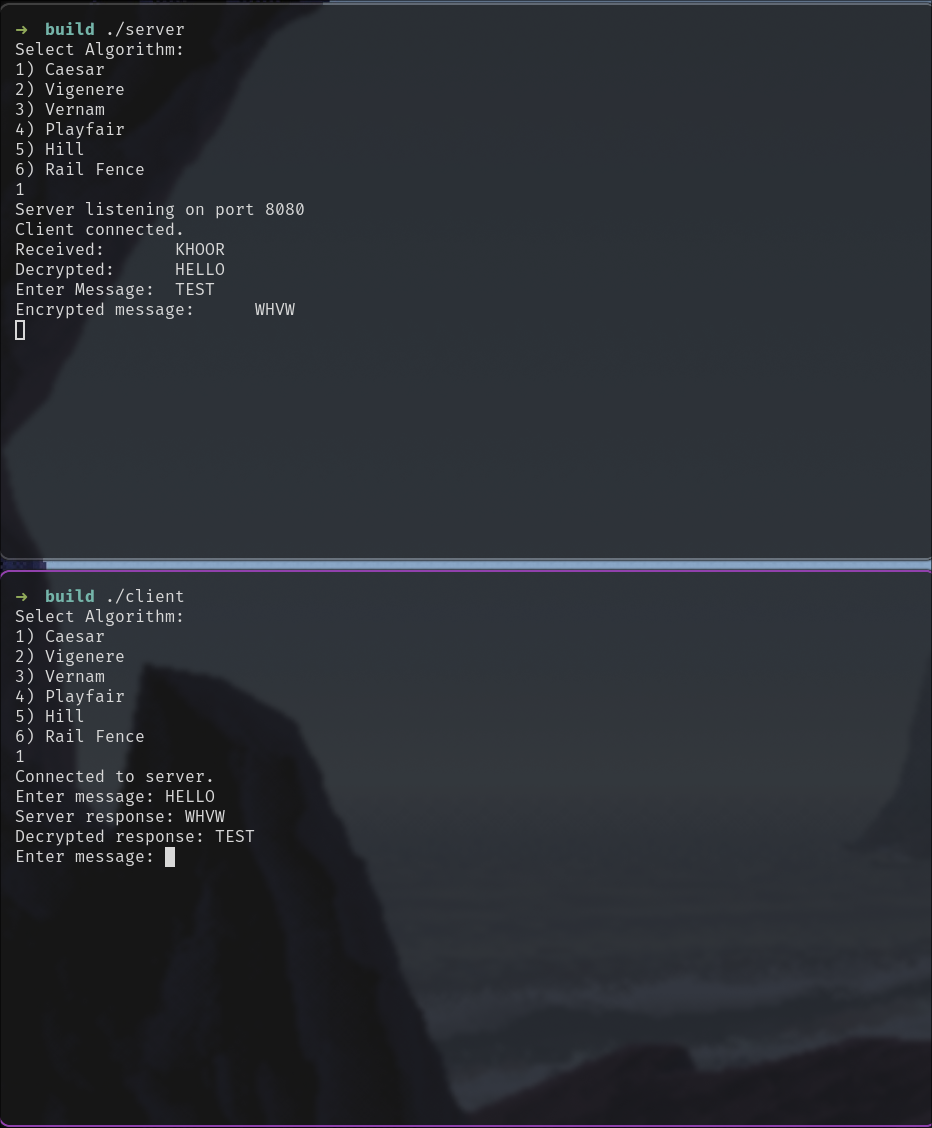
\includegraphics[scale=0.4]{caesar.png}

\subsection{Vigenère Cipher}
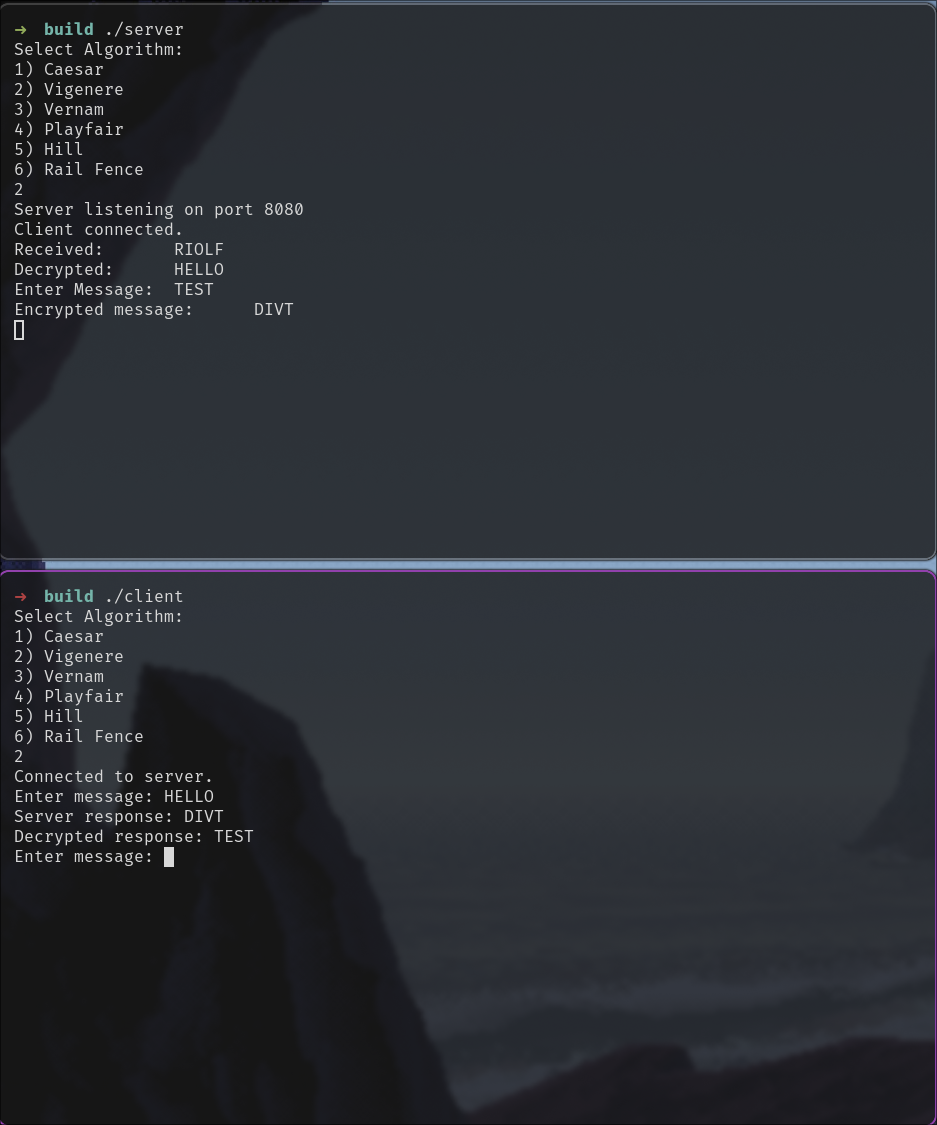
\includegraphics[scale=0.4]{vigenere.png}

\subsection{Vernam Cipher}
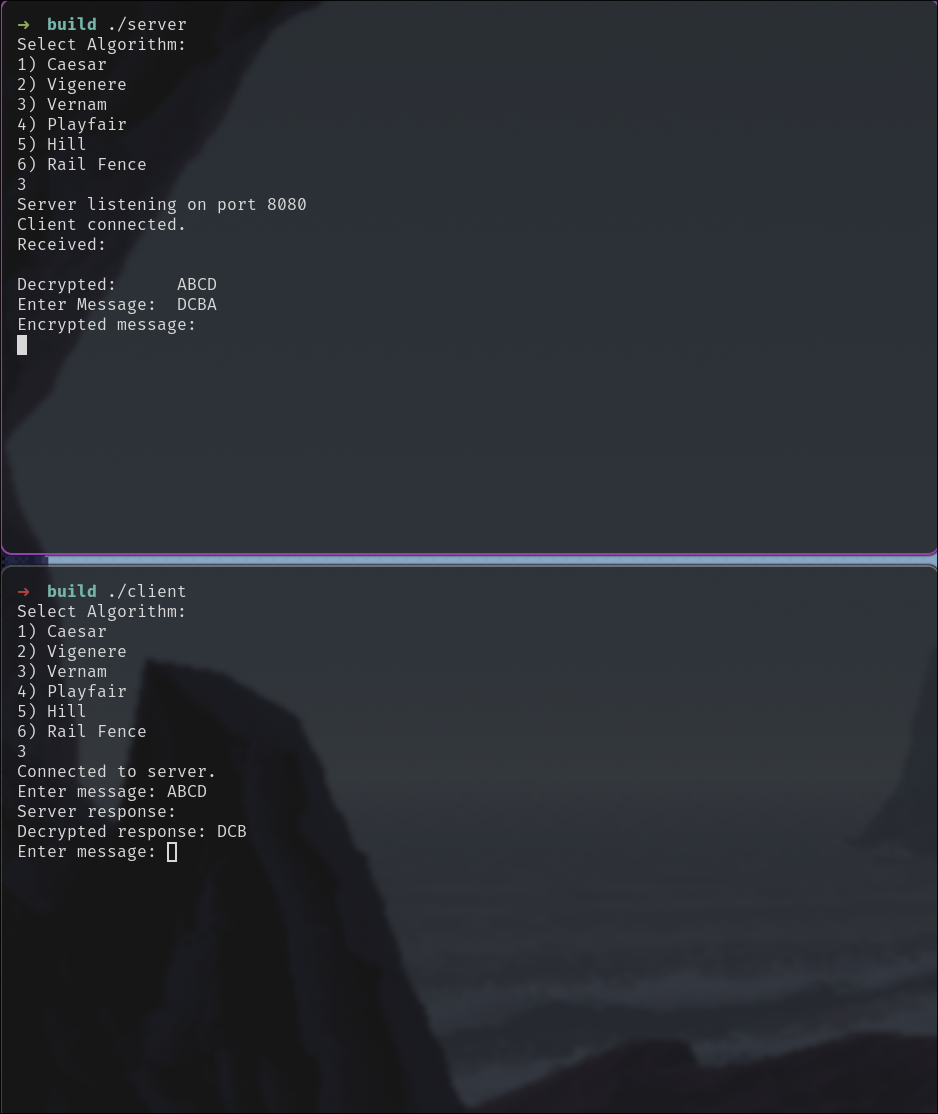
\includegraphics[scale=0.4]{vernam.png}

\subsection{Playfair Cipher}
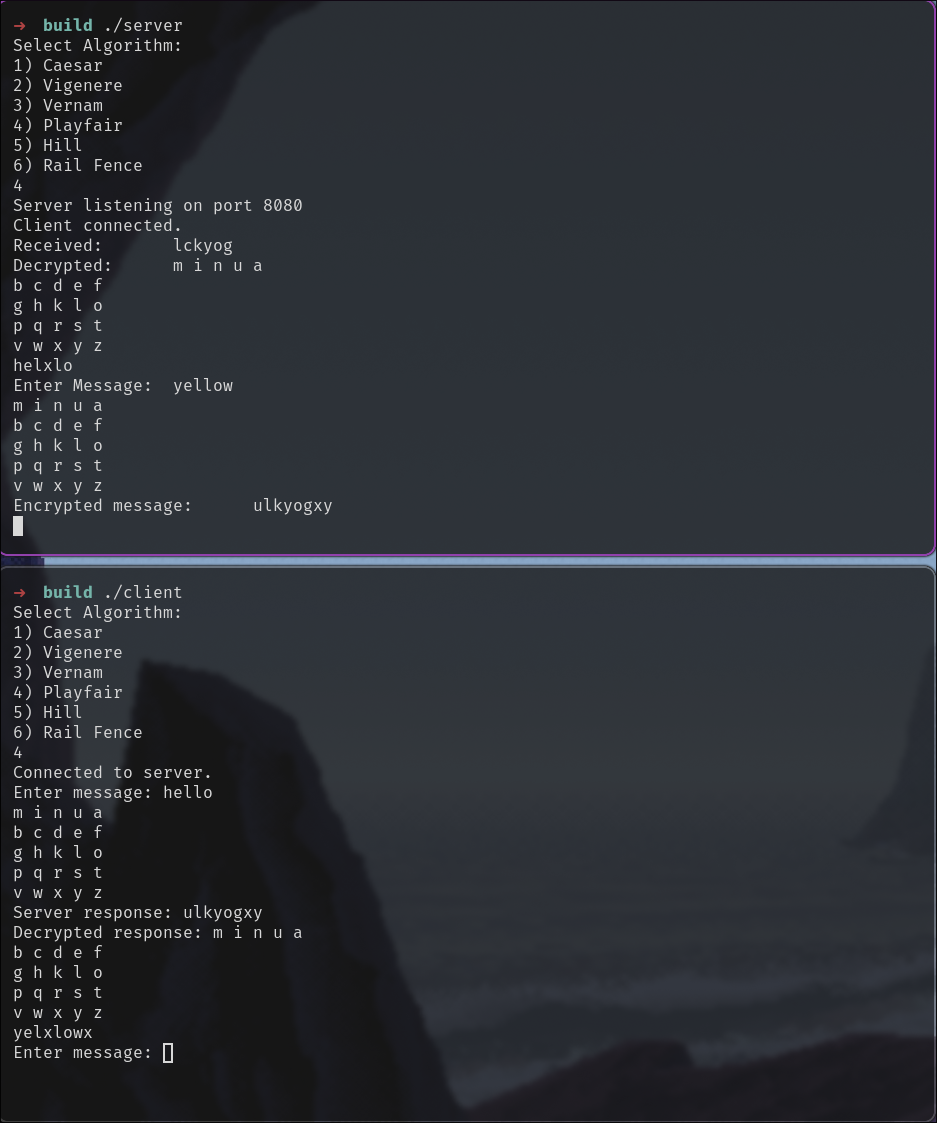
\includegraphics[scale=0.4]{playfair.png}

\subsection{Hill Cipher}
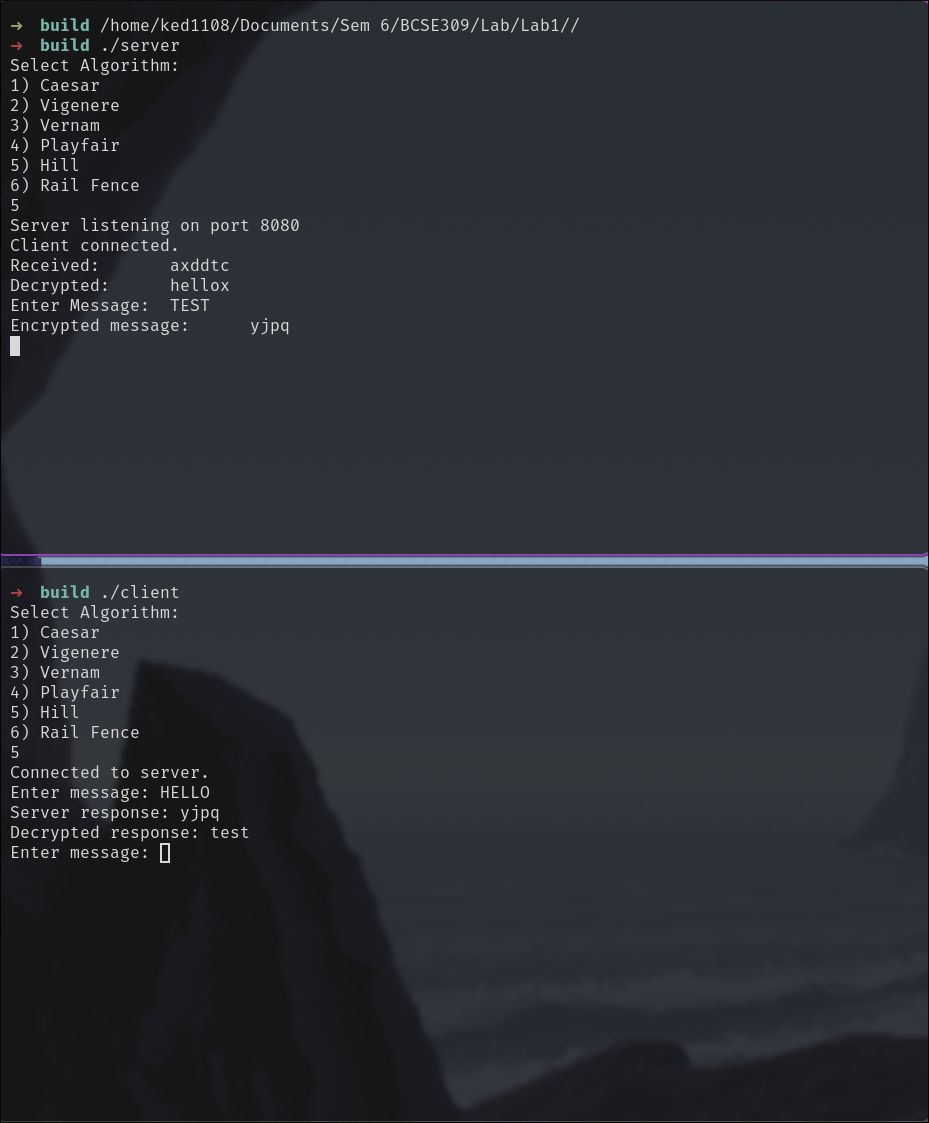
\includegraphics[scale=0.4]{hill.png}

\subsection{Rail Fence Cipher (Columnar Transposition Cipher)}
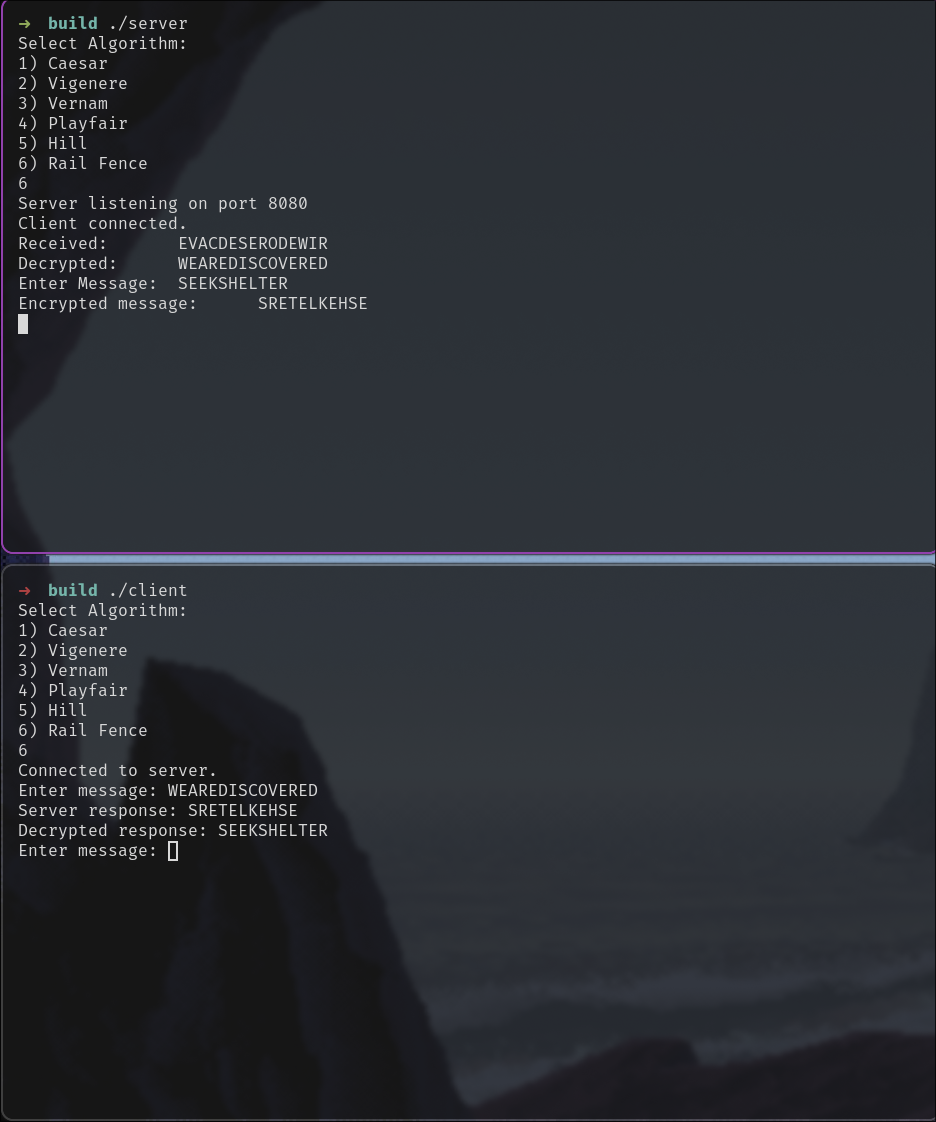
\includegraphics[scale=0.4]{columnar_transposition.png}


\end{document}